\chapter{Float Features}

Examples for floats were already shown in \cref{fig:censorbox,tab:main_font_examples}.
These are handled by the packages \ctanpackage{caption} and \ctanpackage{floatrow}.
A notable feature is the capability for captions the same width as the float they are attached to.
This tends to look much tighter and tidier, see
\cref{fig:wide_caption,fig:tighter_caption} for a comparison.

\begin{figure}\ContinuedFloat*% Floats can be "continued" across pages like this
    % Conventional figure-syntax
    \includesvg[width=0.4\textwidth]{compressor_impeller_isometric}%
    \caption{%
        Example for a regular caption,
        spanning the whole width since it is so long.
        This can quickly look strange, especially if the figure itself is narrow%
    }%
    \label{fig:wide_caption}%
\end{figure}

\begin{figure}\ContinuedFloat
    % Optional argument \FBwidth causes graphic to be its actual size and caption
    % to take up the remaining space. Otherwise, horizontal space is split 50/50,
    % which doesn't make much sense.
    \ffigbox[\FBwidth]{%
        \caption{
            Example for a new caption, spanning the just the width of the float
            it is attached to, despite its length%
        }%
        \label{fig:tighter_caption}%
    }{%
        \includesvg[width=0.4\textwidth]{compressor_impeller_isometric}%
    }%
\end{figure}

\subsubsection{Multiple floats}

Other possibilities are rather arbitrary arrangements of sub\-/figures and -captions.
For this, see \cref{fig:multiple_floats}, which contains the two sub\-/figures
\cref{fig:multiple_floats_one,fig:multiple_floats_two}.
Multiple sub\-/tables are also possible, see \cref{tab:multiple_tables} with its four
sub\-/tables
\cref{tab:multiple_tables_one,tab:multiple_tables_two,tab:multiple_tables_three,tab:multiple_tables_four}.

\begin{figure}
    \ffigbox[\FBwidth]{%
        \begin{subfloatrow}[2]% Default is 2
            \ffigbox[\FBwidth]{%
                \includesvg[width=0.4\textwidth]{rotor_tip_clearance}
            }{%
                \caption{An example}%
                \label{fig:multiple_floats_one}%
            }%
            \ffigbox[\FBwidth]{%
                \includesvg[width=0.4\textwidth]{gas_volume}
            }{%
                \caption{Another example}%
                \label{fig:multiple_floats_two}%
            }%
        \end{subfloatrow}
    }{%
        \caption{%
            An example for sub\-/figures%
        }%
        \label{fig:multiple_floats}%
        \floatfoot{%
            This field can be used for a reference to a source:
            \adaptedfrom{} wherever%
        }%
    }%
\end{figure}

\begin{table}
    \small
    \floatbox{table}{
        %https://tex.stackexchange.com/q/295567/120853
        \begin{subfloatrow}
            \ttabbox[\FBwidth]{%
                \begin{tabular}{
                    @{}
                    m{0.25\textwidth}
                    m{0.15\textwidth}
                    @{}
                }
                    \toprule
                        Column One & Column Two\\
                    \midrule
                        Just & a \\
                        normal & table\\
                        Nothing & special.\\
                    \bottomrule
                \end{tabular}
            }{%
                \caption{Table One}%
                \label{tab:multiple_tables_one}%
            }%
            %
            \ttabbox[\FBwidth]{%
                \begin{tabular}{
                    @{}
                    m{0.25\textwidth}
                    m{0.15\textwidth}
                    @{}
                }
                    \toprule
                        Column One & Column Two\\
                    \midrule
                        Just & a \\
                        normal & table\\
                        Nothing & special.\\
                    \bottomrule
                \end{tabular}
            }{%
                \caption{Table Two}%
                \label{tab:multiple_tables_two}%
            }%
            %
        \end{subfloatrow}
        \vspace{1.5\baselineskip}%

        \begin{subfloatrow}
            \ttabbox[\FBwidth]{%
                \begin{tabular}{
                    @{}
                    m{0.25\textwidth}
                    m{0.15\textwidth}
                    @{}
                }
                    \toprule
                        Column One & Column Two\\
                    \midrule
                        Just & a \\
                        normal & table\\
                        Nothing & special.\\
                    \bottomrule
                \end{tabular}
            }{%
                \caption{Table Three}%
                \label{tab:multiple_tables_three}%
            }%
            %
            \ttabbox[\FBwidth]{%
                \begin{tabular}{
                    @{}
                    m{0.25\textwidth}
                    m{0.15\textwidth}
                    @{}
                }
                    \toprule
                        Column One & Column Two\\
                    \midrule
                        Just & a \\
                        normal & table\\
                        Nothing & special.\\
                    \bottomrule
                \end{tabular}
            }{%
                \caption{Table Four}%
                \label{tab:multiple_tables_four}%
            }%
            %
        \end{subfloatrow}
    }{%
        \caption{%
            Example for multiple tables in one float%
        }%
        \label{tab:multiple_tables}%
    }%
\end{table}

\subsubsection{Side-Captions}

Occasionally, figures and their captions can look disproportionate in combination.
In these cases, placing a side\-/caption might relieve the situation,
as shown in \cref{fig:sidecap}.
\begin{figure}
    \fcapside[\FBwidth]{%
        \caption{%
            A side caption, which may also span multiple lines like demonstrated
            in this rather long caption right here%
        }
        \label{fig:sidecap}%
    }{%
        \includesvg[width=0.6\textwidth]{compressor_rotating_stall}%
    }%
\end{figure}

\subsubsection{Large Floats}

An example for a larger table is shown in \cref{tab:fuel_composition}.
One key aspect there: the \verb|S| column\-/type, provided by \ctanpackage{siunitx}.
It automatically applies \verb|\num| to each cell, which in turn allows easy
printing of things like: \num{-3.23e-5}.
Further, decimal places are accounted for and aligned by automatically.
Use \verb|*x{y}| to print column-type \verb|y| (\iecfeg{i.e.}\ \verb|c|) \verb|x|
times.
No need for tedious repetition.

\begin{landscape}
    \begin{table}
        \crefname{equation}{eq.}{eqs.}% Keep this change scoped to the environment
        \Crefname{equation}{Eq.}{Eqs.}%
        \footnotesize%
        \ttabbox{%
            \caption{%
                Compositions and properties of fuels, as used in \Cref{eq:tikz_in_text}%
            }%
            \label{tab:fuel_composition}%
        }{%
            \begin{tabular}{
                @{}
                p{5em}
                *7{S[table-format=1.4]}
                S[table-format=4.0]
                S[table-format=2.1]
                @{}
            }
                \toprule
                    Name &
                        \multicolumn{7}{c}{{Mass fraction \(\sym{mass_fraction}\)}} &
                        {\(\sym{density}\)} &
                        {\(\sym{heating_value}\)}
                    \\
                    &
                        \multicolumn{7}{c}{{[--]}} &
                        \(\brackets*{\si{\kilogram\per\meter\cubed}}\) &
                        \(\brackets*{\si{\mega\joule\per\kilogram}}\)
                    \\
                \cmidrule(lr){2-8}% truncate left and right
                    &
                        \chcpd{C} &
                        \chcpd{H} &
                        \chcpd{S} &
                        \chcpd{O} &
                        \chcpd{N} &
                        \chcpd{H2O} &
                        {Ash} & % Escape text from S-column using braces
                        &
                    \\
                \midrule
                    Diesel\mpfootnotemark[1] &
                        0.8600 &
                        0.1320 &
                        0.0060 &
                        \multicolumn{2}{c}{\num{0.0020}\mpfootnotemark[2]} &
                        {n.a.} &
                        {n.a.} &
                        840 &
                        42.7
                    \\
                    Oil EL\mpfootnotemark[1] &
                        0.8570 &
                        0.1310 &
                        0.0100 &
                        \multicolumn{2}{c}{\num{0.0020}\mpfootnotemark[2]} &
                        {n.a.} &
                        {n.a.} &
                        840 &
                        42.7
                    \\
                    Oil H\mpfootnotemark[1] &
                        0.8490 &
                        0.1060 &
                        0.0350 &
                        \multicolumn{2}{c}{\num{0.0100}\mpfootnotemark[2]} &
                        {n.a.} &
                        {n.a.} &
                        980 &
                        40.0
                    \\
                    \abb{marine_diesel_oil}\mpfootnotemark[3] &
                        {n.a.} &
                        {n.a.} &
                        0.0150 &
                        {n.a.} &
                        {n.a.} &
                        0.0030\mpfootnotemark[4] &
                        0.0001 &
                        900 &
                        {n.a.}
                    \\
                    \abb{heavy_fuel_oil}\mpfootnotemark[5] &
                        {n.a.} &
                        {n.a.} &
                        0.0350\mpfootnotemark[6] &
                        {n.a.} &
                        {n.a.} &
                        0.0050\mpfootnotemark[4] &
                        0.0015 &
                        1010 &
                        {n.a.}
                    \\
                \addlinespace
                    Light\mpfootnotemark[7] &
                        0.8600 &
                        0.1320 &
                        0.0060 &
                        0.0010 &
                        0.0010 &
                        0 &
                        0 &
                        840 &
                        {\Cref{eq:boie}}
                    \\
                    Medium\mpfootnotemark[7] & 
                        0.8530 &
                        0.1269 &
                        0.0150 &
                        0.0010 &
                        0.0010 &
                        0.0030 &
                        0.0001 &
                        900 &
                        {\Cref{eq:boie}}
                    \\
                    Heavy\mpfootnotemark[7] &
                        0.8460 &
                        0.1025 &
                        0.0350 &
                        0.0050 &
                        0.0050 &
                        0.0050 &
                        0.0015 &
                        1010 &
                        {\Cref{eq:boie}}
                    \\
                \bottomrule
            \end{tabular}%
            % Unfortunately, these have to be numbered manually.
            % Float/table footnotes are a touchy topic, and this was chosen as the
            % least worst approach out of the alternatives.
            \footnotetext[1]{%
                \cite[634]{baehr_thermodynamik:_2016}; see also
                \cite[L70]{dubbel_taschenbuch_2007} and
                \cite[97]{mollenhauer_handbuch_2007}.%
            }%
            \footnotetext[2]{%
                Given as a sum
                \(\sym{mass_fraction}_{\chcpd{O}} + \sym{mass_fraction}_{\chcpd{N}}\).%
            }%
            \footnotetext[3]{%
                Max.\ values of specification \emph{DMB},
                \cite{international_organization_for_standardization_iso_2017}.%
            }%
            \footnotetext[4]{%
                Given as a volume fraction, assumed equal to mass fraction.%
            }%
            \footnotetext[5]{%
                Max.\ values of specification \emph{RMK},
                \cite{international_organization_for_standardization_iso_2017}.%
            }%
            \footnotetext[6]{%
                \abb{int_mar_org} level prior to \num{2020}.%
            }%
            \footnotetext[7]{%
                Derived, \emph{virtual} fuels.%
            }%
        }%
    \end{table}%
\end{landscape}

\subsubsection{Table Style}

In general, use the least ink possible to get your point across.
Any more is only noise.
This is especially true for tables.
For this, compare \cref{tab:main_font_examples} with its not\-/so\-/blessed
twin, \cref{tab:main_font_examples_ugly}:
\begin{itemize}
    \item do not use vertical lines in tables,
    \item avoid double lines
    \item if in doubt, left-align.
        If there is no actual reason to center or right\-/align, refrain from it.
\end{itemize}
For more info, see the package \ctanpackage{booktabs}.

\begin{table}
    \ttabbox{%
        \caption{%
            Dreadful version of \cref{tab:main_font_examples}%
        }%
        \label{tab:main_font_examples_ugly}%
    }{%
        \begin{tabular}{
            |
            c
            ||
            c
            |
        }
        \hline
            \textit{Feature} & \textit{Sample Text}\\
        \hline
        \hline
            Regular & \sampletext\\
        \hline
            \textbf{Bold} & \textbf{\sampletext}\\
        \hline
            \textit{Italics} & \textit{\sampletext}\\
        \hline
            \textbf{\textit{Bold Italics}} & \textbf{\textit{\sampletext}}\\
        \hline
            \textsc{Small Capitals} & \textsc{\sampletext}\\
        \hline
            \textbf{\textsc{Bold SC}} & \textbf{\textsc{\sampletext}}\\
        \hline
            \textit{\textsc{Italics SC}} & \textit{\textsc{\sampletext}}\\
        \hline
        \end{tabular}
    }%
\end{table}

\subsubsection{Caption Positioning}

Note that table captions (see for example \cref{tab:multiple_tables}) occur
\emph{above} the table no matter the \verb|\caption| command's position in
the source code.
Per convention, figure captions should appear below, table captions above their bodies.
This is handled automatically by \ctanpackage{floatrow}.
Also note that there is neither a period nor \emph{any} character
(no space, no empty line) behind the last caption line in the source code,
since those periods are managed globally by the \ctanpackage{caption} package.
They can therefore be toggled easily.

\paragraph{Float Footer}
There is also a \verb|\floatfoot| command for all floats.
This is used to place additional info underneath the caption, for example for
references, \iecfeg{cf.}\ \cref{fig:multiple_floats}.

\section{TikZ and pgfplots}
Packages \ctanpackage{tikz} and \ctanpackage{pgfplots} offer a vast array of features.
A select few are presented here.

\subsection{Drawing over Bitmaps}
When having to rely on bitmaps, one might still want to add additional info.
This can be done directly in \LaTeX{}, profiting from all the usual features.
In the example here, this is of course the retaining of the text font, but also
employing the useful \ctanpackage{contour} package to draw legible black\-/on\-/white
(or vice\-/versa) text.
An example is shown in \cref{fig:bitmap_tikz}.
There is a debugging grid functionality to allow for easier positioning of the labels
on the graphic.
\cref{fig:bitmap_tikz} also showcases a vertical alignment of sub\-/figures.

\begin{figure}
    \ffigbox[\FBwidth]{%
        \begin{subfloatrow}
        \hsize1\textwidth
        \vbox{
            \ffigbox[\FBwidth]{
                \begin{tikzpicture}[%
                    every node/.style={
                        font=\footnotesize
                    }
                ]
                    \node[anchor=south west,inner sep=0] (image) at (0,0) {
                        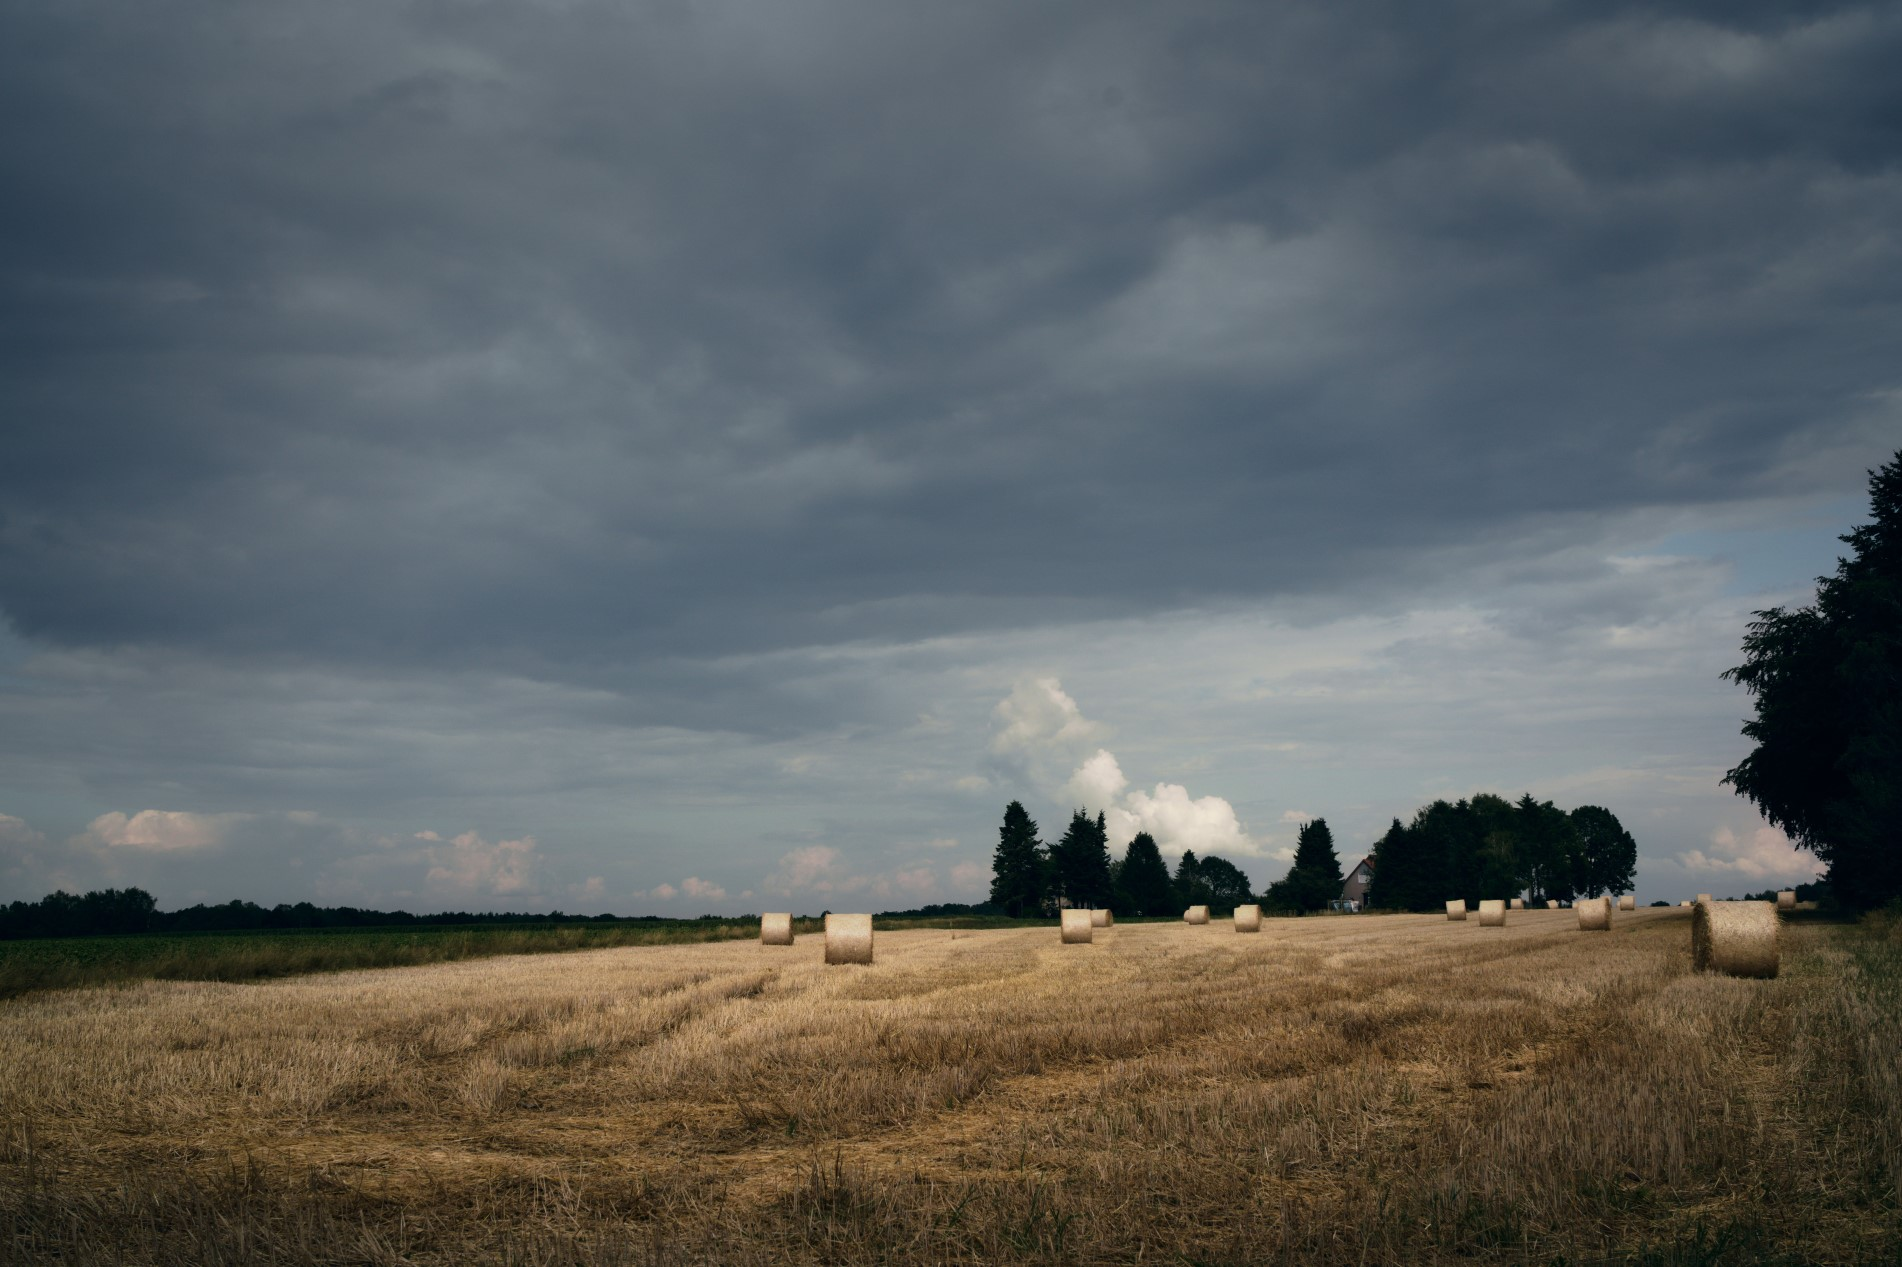
\includegraphics[width=0.7\textwidth]{field}
                    };
                    \begin{scope}[x={(image.south east)},y={(image.north west)}]

                        % All floating descriptions:
                        \foreach \x/\y/\nodetext in {
                            0.50/0.20/{A field!},
                            0.50/0.70/{The sky!}%
                        }{
                            \node at (\x,\y) {\ctrw{\nodetext}};
                        }

                        \draw[annotationarrow] (0.75,0.45) -- (1.05,0.50)
                            node[align=left, right, text width=5em] {An annotation!};

                        % DEBUGGING COMMAND
                        \debugtikzsvg
                    \end{scope}
                \end{tikzpicture}
            }{
                \caption{Debugging/positioning grid}
                \label{fig:bitmap_tikz_debug}
            }%
            \vss
            \vspace{3ex}

            \ffigbox[\FBwidth]{
                \begin{tikzpicture}[%
                    every node/.style={
                        font=\footnotesize
                    }
                ]
                    \node[anchor=south west,inner sep=0] (image) at (0,0) {
                        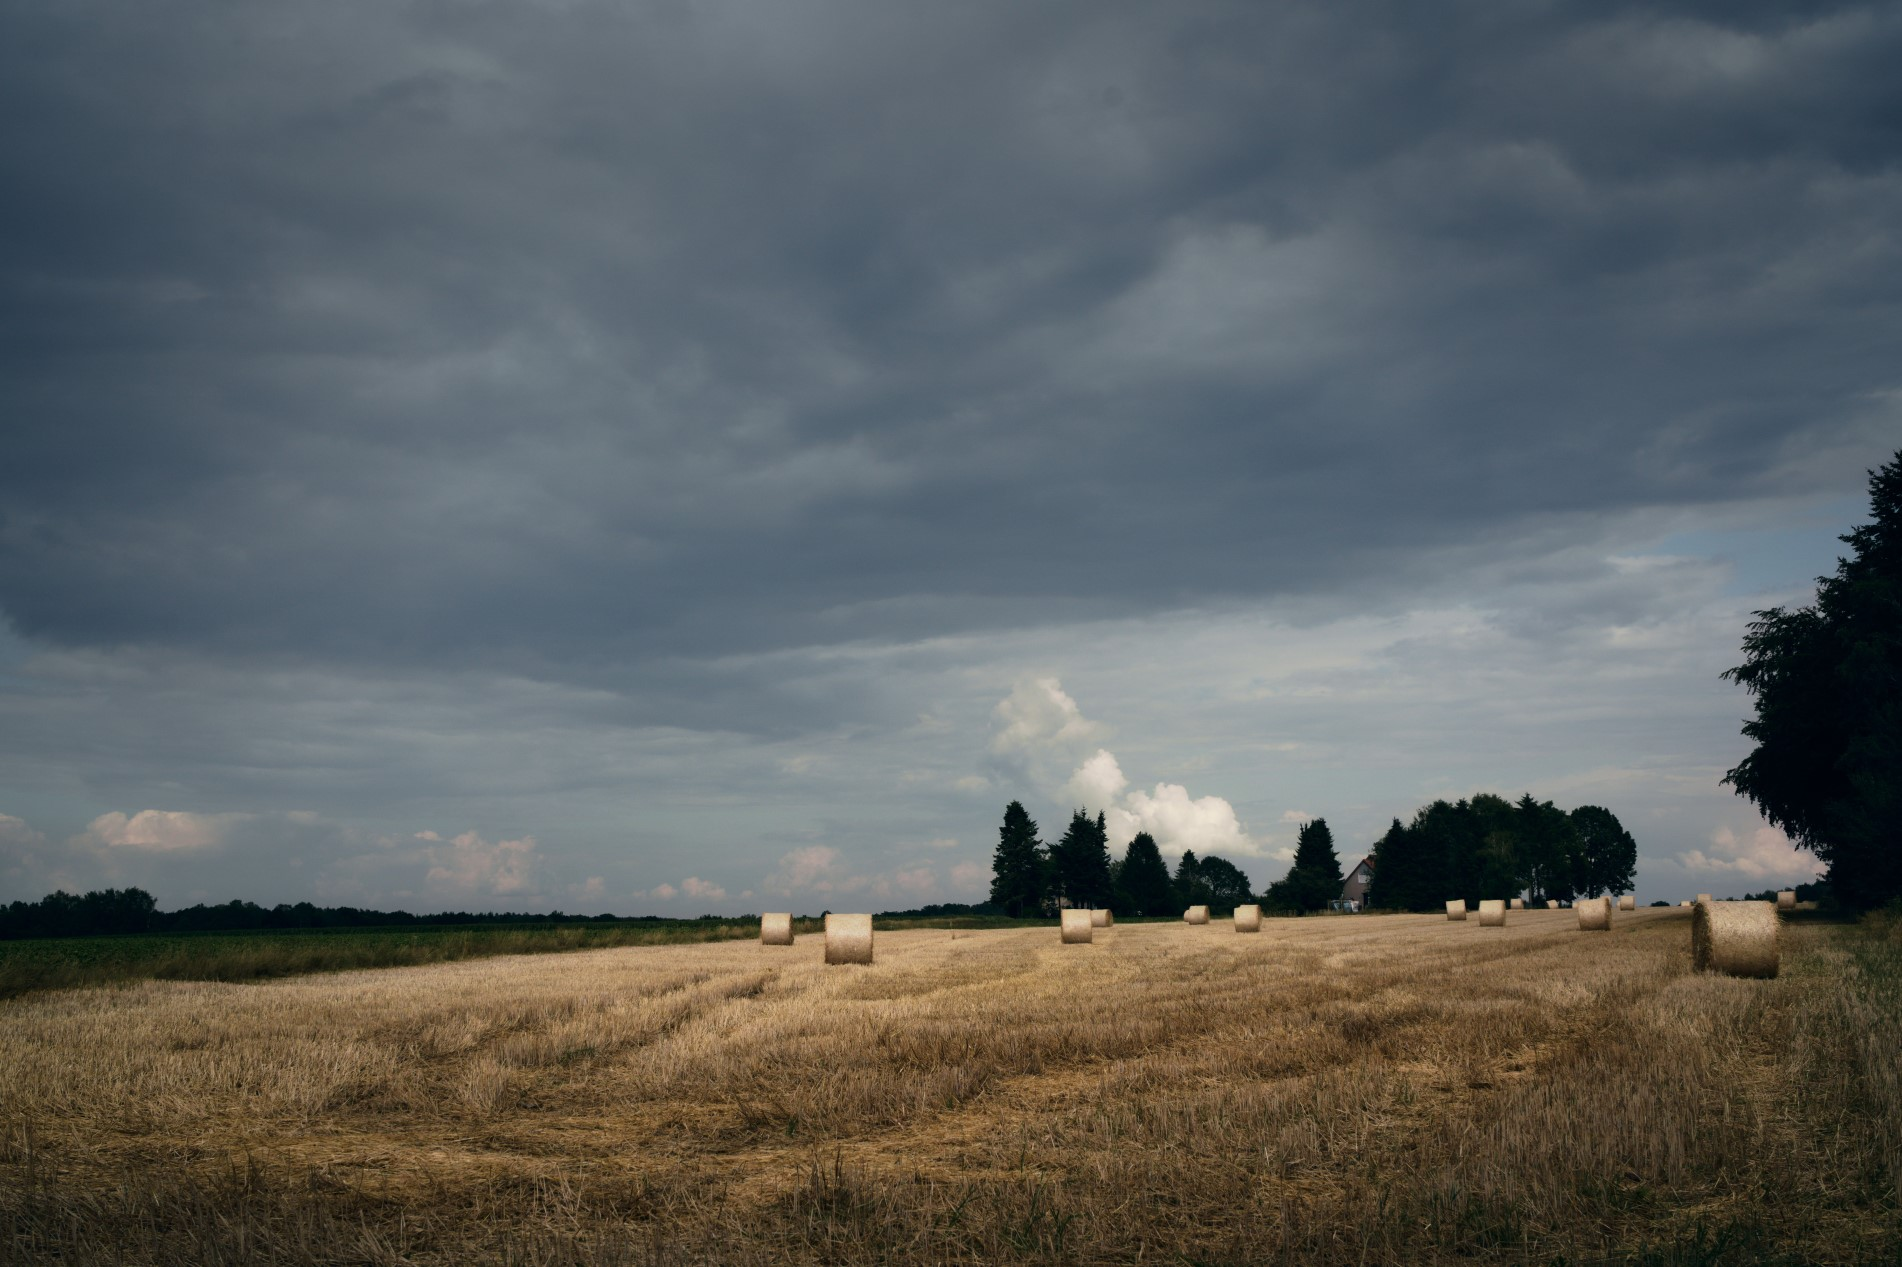
\includegraphics[width=0.7\textwidth]{field}
                    };
                    \begin{scope}[x={(image.south east)},y={(image.north west)}]

                        % All floating descriptions:
                        \foreach \x/\y/\nodetext in {
                            0.50/0.20/{A field!},
                            0.50/0.70/{The sky!}%
                        }{
                            \node at (\x,\y) {\ctrw{\nodetext}};
                        }

                        \draw[annotationarrow] (0.75,0.45) -- (1.05,0.50)
                            node[align=left, right, text width=5em] {An annotation!};

                        % DEBUGGING COMMAND
                        % \debugtikzsvg
                    \end{scope}
                \end{tikzpicture}
            }{
                \caption{Result}
                \label{fig:bitmap_tikz_result}
            }
        }
        \end{subfloatrow}
    }{%
        \caption{%
            Drawing over a bitmap graphic using Ti\textit{k}Z in a vertical sub\-/figure
            environment%
        }
        \label{fig:bitmap_tikz}
    }
\end{figure}

\subsection{Plotting}

If you rely on tools like \texttt{matlab2tikz}, this is for you.
Instead of these outside tools, one can plot \emph{directly} in \LaTeX{}, either
through importing external \texttt{*.csv} data (for example from experiments)
or through computing the plots using \ctanpackage{pgfplots} directly from within
\LaTeX{}.

\subsubsection{Directly in \LaTeX{}}
Plotting and computing the return values directly in \LaTeX{} is achieved through
the \texttt{declare function} command.
While the functionality is limited (owed to the limitations of \TeX{}, which is
of course not meant for this sort of thing),
it may still save a lot of time and headaches.
Finding and specifying the correct settings for \ctanpackage{pgfplots} can take
a lot of time.
This is already taken care of for this document.
As such, a plot from existing \texttt{*.csv} data can be set up in a handful of
lines using one of the built-in styles, like \texttt{regularplot}.
Plotting from a Ti\textit{k}Z function is demonstrated in
\cref{fig:plotting_in_latex,fig:plotting_in_latex_tufte}.

\tikzset{
    declare function={% https://tex.stackexchange.com/a/279234/120853
        % SHOMATE equation for air w/ N2/O2/Ar/CO2.
        % This is needlessly complex and verbose, but showcases some interesting
        % features, like conditionals for piecewise functions.
        cpm(\x)=%
            (\x<=500) *% Below 500 degC
                (
                    0.781 *% N2
                    (
                        28.98641+1.853978*((\x+273.15)/1000)
                        -
                        9.647459*((\x+273.15)/1000)^2
                        +
                        16.63537*((\x+273.15)/1000)^3
                        +
                        0.000117/(((\x+273.15)/1000)^2)
                    )
                    +
                    0.2093 *% O2
                    (
                        31.32234-20.23531*((\x+273.15)/1000)
                        +
                        57.86644*((\x+273.15)/1000)^2
                        -
                        36.50624*((\x+273.15)/1000)^3
                        -
                        0.007374/((\x+273.15)/1000)^2
                    )
                    +
                    0.0093 *% Ar
                    (
                        20.78600+2.825911e-7*((\x+273.15)/1000)
                        -
                        1.464191e-7*((\x+273.15)/1000)^2
                        +
                        1.092131e-8*((\x+273.15)/1000)^3
                        -
                        3.661371e-8/((\x+273.15)/1000)^2
                    )
                    +
                    0.0004 *% CO2
                    (
                        24.99735+55.18696*((\x+273.15)/1000)
                        -
                        33.69137*((\x+273.15)/1000)^2
                        +
                        7.948387*((\x+273.15)/1000)^3
                        -
                        0.136638/((\x+273.15)/1000)^2
                    )
                )
            +
            (\x>500) *% Above 500 degC
                (
                    0.781 *% N2
                    (
                        19.50583+19.88705*((\x+273.15)/1000)
                        -
                        8.598535*((\x+273.15)/1000)^2
                        +
                        1.369784*((\x+273.15)/1000)^3
                        +
                        0.527691/(((\x+273.15)/1000)^2)
                    )
                    +
                    0.2093 *% O2
                    (
                        31.32234-20.23531*((\x+273.15)/1000)
                        +
                        57.86644*((\x+273.15)/1000)^2
                        -
                        36.50624*((\x+273.15)/1000)^3
                        -
                        0.007374/((\x+273.15)/1000)^2
                    )
                    +
                    0.0093 *% Ar
                    (
                        20.78600+2.825911e-7*((\x+273.15)/1000)
                        -
                        1.464191e-7*((\x+273.15)/1000)^2
                        +
                        1.092131e-8*((\x+273.15)/1000)^3
                        -
                        3.661371e-8/((\x+273.15)/1000)^2
                    )
                    +
                    0.0004 *% CO2
                    (
                        24.99735+55.18696*((\x+273.15)/1000)
                        -
                        33.69137*((\x+273.15)/1000)^2
                        +
                        7.948387*((\x+273.15)/1000)^3
                        -
                        0.136638/((\x+273.15)/1000)^2
                    )
                );
    }%
}

\begin{figure}\ContinuedFloat*
    \ffigbox[\FBwidth]{%
        \caption{%
            Caloric parameters of air.
            \textbf{Avoid legends} and put info where it belongs,
            improving legibility (less back-and-forth for the eye).
            This plot is using the custom \texttt{regularplot} style%
        }%
        \label{fig:plotting_in_latex}%
    }{%
        \begin{tikzpicture}
            \begin{axis}[%
                regularplot,%
                axis y line*=right,%
                axis x line=none,%
                grid=none,% Grid can only be on one side
                % Using \ensuremath{} for each symbol, no need to use math mode here
                ylabel={\sym{ratio_of_specific_heats}},
                y unit={-},
            ]
                \addplot+[domain=20:400]{cpm(x)/(cpm(x)-8.3145)}
                    node [arrowlabel=0.3, sloped]
                        {\sym{ratio_of_specific_heats}};
            \end{axis}
            \begin{axis}[% https://tex.stackexchange.com/a/31504/120853
                regularplot,%
                xlabel={\sym{celsius_temperature}},%
                x unit={\degreeCelsius},% This is a siunitx-accepted command
                ylabel={\(\symspec{heat_capacity}_{\sym{pressure}}\)},
                y unit={\joule\per\kilogram\per\kelvin},
                cycle list shift=1,
            ]
                \addplot+[domain=20:400]{cpm(x)/0.0289524}
                    node [arrowlabel=0.3, sloped]
                        {\(\symspec{heat_capacity}_{\sym{pressure}}\)};%
            \end{axis}
        \end{tikzpicture}
    }%
\end{figure}

\begin{figure}\ContinuedFloat
    \ffigbox[\FBwidth]{%
        \caption[Tufte-like plot]{%
            Same content as \cref{fig:plotting_in_latex} in
            \enquote{\emph{\glsentryname{name.edward_tufte}}-like}
            for a modern, minimalist look where precision counts less than
            the overall message.
            For more info, refer to its namesake, \name{edward_tufte}%
        }%
        \label{fig:plotting_in_latex_tufte}
    }{%
        \begin{tikzpicture}
            \begin{axis}[%
                tuftelike,%
                ylabel={\(\symspec{heat_capacity}_{\sym{pressure}}\)},
                y unit = {\joule\per\kilogram\per\kelvin},
                xlabel={\sym{celsius_temperature}},%
                x unit = {\degreeCelsius},
                domain=50:400,
                ymin=1000,
                ymax=1100,
                ytick={1000, 1050, 1100},% Specify manually due to weird rounding
            ]
                \addplot+{cpm(x)/0.0289524}
                    node [arrowlabel=0.3, sloped]
                        {\(\symspec{heat_capacity}_{\sym{pressure}}\)};%
            \end{axis}%
            \begin{axis}[% https://tex.stackexchange.com/a/31504/120853
                tuftelike,%
                axis y line*=right,%
                axis x line=none,%
                ylabel={\sym{ratio_of_specific_heats}},%
                y unit={-},
                cycle list shift=1,
                domain= 50:400,
                ymin=1.35,
                ymax=1.4,
            ]
                \addplot+{cpm(x)/(cpm(x)-8.3145)}
                    node [arrowlabel=0.3, sloped]
                        {\sym{ratio_of_specific_heats}};
            \end{axis}
        \end{tikzpicture}
    }%
\end{figure}

\subsubsection{Importing CSV}

Often, one wants to plot data from files.
The better behaved the file is (meaningful headers, no junk rows), the easier that is.
In \cref{fig:diffuser}, \verb|y=<column header>| is all that has to be specified for the
column corresponding to that name to be automatically chosen, with no confusion
about indices or column numbers.
\begin{figure}
\ffigbox[\FBwidth]{
        \caption{Plotting from CSV data for a diffuser}
        \label{fig:diffuser}
    }{%
        \pgfplotstableread{data/diffuser.csv}{\diffusertable}%
        \begin{tikzpicture}
            \begin{axis}[%
                tuftelike,%
                axis y line*=left,%
                xlabel={\(\sym{radius}/\sym{radius}_{\num{2}}\)},%
                x unit={-},
                ylabel={
                    \sym{mach_number},
                    \(\sym{pressure}/\sym{pressure}_{\num{2}}\),
                    \(\sym{abs_temperature}/\sym{abs_temperature}_{\num{2}}\),
                    \(\sym{density}/\sym{density}_{\num{2}}\)
                },%
                y unit={-},
                table/x={R_pres},%
                ymin=0.4,
                ymax=1.3,
                ytick={0.4, 0.7, 1, 1.3},
                xmin=1,
                xmax=1.6
            ]%
                % Do this manually, node macro expansion in foreach/invokeforeach
                % is error-prone
                \addplot+ table [y=M] {\diffusertable}
                    node [arrowlabel=0.2]
                    {\sym{mach_number}};
                \addplot+ table [y=Pi] {\diffusertable}
                    node [arrowlabel=0.9]
                    {\(\sym{pressure}/\sym{pressure}_{\num{2}}\)};
                \addplot+ table [y=Theta] {\diffusertable}
                    node [arrowlabel=0.7]
                    {\(\sym{abs_temperature}/\sym{abs_temperature}_{\num{2}}\)};
                \addplot+ table [y=Rho] {\diffusertable}
                    node [arrowlabel=0.8]
                    {\(\sym{density}/\sym{density}_{\num{2}}\)};
            \end{axis}%
            %
            \begin{axis}[%
                tuftelike,%
                axis y line*=right,%
                axis x line=none,%
                ylabel={abs.\ flow angle \sym{angle_one}},%
                y unit={\degree},
                cycle list shift=4,%
                ymin=13,
                ymax=15,
                xmin=1,
                xmax=1.6,
            ]%
                \addplot+ table [x=R_pres, y=alpha] {\diffusertable}
                    node [arrowlabel] {\sym{angle_one}};%
            \end{axis}%
        \end{tikzpicture}
    }
\end{figure}

\subsection{Tikz and Text}

Ti\textit{k}Z content can also be intertwined with text using \verb|\tikzmark|.
This is illustrated in \cref{eq:tikz_in_text}.
Note that this procedure needs two compilation runs, since the label positions
need to be written to an auxiliary file first.

\begin{minipage}{1\linewidth}
    % https://tex.stackexchange.com/q/83746/120853 and
    % https://tex.stackexchange.com/a/188221/120853
    \newcommand*{\setmuskip}[2]{#1=#2\relax}
    \setmuskip{\medmuskip}{15mu plus 2mu minus 4mu}
    \setmuskip{\thickmuskip}{18mu plus 2mu minus 4mu}

    \begin{equation}\label{eq:tikz_in_text}
        \tikzmark{c}\sym{mass_fraction}_{\chcpd{C}}
        +
        \tikzmark{h}\sym{mass_fraction}_{\chcpd{H}}
        +
        \tikzmark{s}\sym{mass_fraction}_{\chcpd{S}}
        +
        \tikzmark{o}\sym{mass_fraction}_{\chcpd{O}}
        +
        \tikzmark{n}\sym{mass_fraction}_{\chcpd{N}}
        +
        \tikzmark{w}\sym{mass_fraction}_{\chcpd{H2O}}
        +
        \tikzmark{a}\sym{mass_fraction}_{\mathrm{ash}}
        \coloneq% prints as :=
        \num{1}
        \eqend{}
    \end{equation}

    \begin{tikzpicture}[%
        remember picture,%
        overlay,%
    ]
        \pgfmathsetmacro{\vshiftone}{4}
        \pgfmathsetmacro{\vshifttwo}{6.5}
        \pgfmathsetmacro{\vshiftthree}{9}
        \pgfmathsetmacro{\hshiftone}{1}
        \pgfmathsetmacro{\hshifttwo}{2}
        \pgfmathsetmacro{\hshiftthree}{3}

        \foreach \x/\y/\a/\b in {%
            c/Carbon/\vshiftone/-\hshiftthree,%
            h/Hydrogen/\vshifttwo/-\hshifttwo,%
            s/Sulphur/\vshiftthree/-\hshiftone,%
            o/Oxygen/\vshifttwo/0,%
            n/Nitrogen/\vshiftthree/\hshiftone,%
            w/Water/\vshifttwo/\hshifttwo,%
            a/Ash/\vshiftone/\hshiftthree%
        }{%
            \node (\x1) [below right=0.1em and 0.4em of pic cs:\x]
                {};
            \node (\x2) [on grid, below right=\a ex and \b ex of \x1, anchor=north]
                % 'on grid' option makes positioning snappy (uses actual middle
                % of nodes); without, even 'right=0pt' would not be centered
                {\y};
            \draw[-stealth] [out=90](\x2) to [in=270](\x1);
        }%
    \end{tikzpicture}

    % We need to use 'overlay', but this also means we lose the bounding box.
    % Eye-ball it here, sadly.
    \vspace{4\baselineskip}
\end{minipage}

\subsection{Regular TikZ pictures}

Ti\textit{k}Z really is not meant for arbitrary graphics.
The more free\-/form images shown in this document were created using InkScape.
Still, \enquote{drawing} in Ti\textit{k}Z is much preferred and easier when the
images are somewhat programmatic, aka there are straight corners, edges and turns,
equal distances, and everything is a bit \enquote{block-like}, repetitive.
For example, a small file structure diagram:
\begin{center}
    \begin{tikzpicture}[
        %http://www.texample.net/tikz/examples/filesystem-tree/
            grow via three points={one child at (0.5,-0.7) and
                two children at (0.5,-0.7) and (0.5,-1.4)},
            edge from parent path={(\tikzparentnode.south) |- (\tikzchildnode.west)},
            every node/.style={draw=black,thick,anchor=west,fill=g5},
            font=\ttfamily,%
        ]%
            \node {\faFileO{} parent.py}
            child { node {\faFileO{} constants.py}}
            child { node {\faFileO{} parameters.py}}
            child { node {\faFileO{} handling.py}}
            child { node {\faFileO{} performance\_maps.py}};
    \end{tikzpicture}
\end{center}
Note how \verb|tikzpicture| environments do not have to be contained in floats.

A second Ti\textit{k}Z example is shown in \cref{fig:tikz_diagram}.

\begin{figure}
    \ffigbox[0.95\linewidth]{%
        \begin{tikzpicture}[%
            every path/.style={thick},%https://tex.stackexchange.com/a/302931/120853
            simblock/.style={%
                draw,%
                line width=1.5pt,%
                minimum size=1.5em,%
                rounded corners,%
                fill=white,%
            },%
            triangle/.style={%
                regular polygon,%
                regular polygon sides=3,%
                inner sep=0.2ex,% Fit tightly
                outer sep=0pt,
            },
        ]%
        % Row of Model Blocks
            \node[simblock, minimum height=5ex] (outlet)
                {Outlet};
            \node[simblock, minimum height=5ex, right=of outlet] (turbine)
                {Turbine};
            \node[simblock, minimum height=5ex, right=of turbine] (compressor)
                {Compressor};
            \node[simblock, minimum height=5ex, right=of compressor] (inlet)
                {Inlet};
            \draw[->] (outlet) -- (turbine)
                node [midway, above, font=\footnotesize] {feeds};
            \draw[->] (turbine) -- (compressor)
                node [midway, above, font=\footnotesize, align=center] (shaft) {via\\shaft};
            \draw[->] (compressor) -- (inlet)
                node [midway, above, font=\footnotesize] {feeds};

            % Division Block underneath Engine
            \node[below=12ex of inlet.south, draw=none] (div) {};
            \node[below=4ex of div, draw=none] (mult) {};
            \node[simblock, fit=(mult) (div), minimum height=8ex] (multdiv) {};
            \node at (div) {\(\div\)};
            \node at (mult) {\(\ast\)};

            % Connect Inlet and Division part
            \draw[->] (inlet.east) -- ++ (+1, 0)
                node [pos=1, above] {\(p_{\text{in}}(\tau)\)}
                |-
                ($(multdiv.east)!0.5!(multdiv.north east)$);

            % p min block next to multiplication
            \draw[<-] ($(multdiv.east)!0.5!(multdiv.south east)$) -- ++ (1, 0)
                node[simblock] {\(p\)};

            \node [circle, fill, inner sep=0.3ex, left=0.7em of multdiv] (split1) {};
            \draw (multdiv) -- (split1);

            % Bias and inverted Bias blocks
            \node[simblock, left = of div] (biasinv) {\(1 - u\)};
            \node[simblock, left = of mult] (bias) {\(u - 1\)};
            \draw[->] (split1) |- (bias);
            \draw[->] (split1) |- (biasinv);

            % Split again
            \node [circle, fill, inner sep=0.3ex, left=1em of biasinv] (split2) {};
            \draw (biasinv) -- (split2);

            \node[simblock, left=1em of split2, triangle, shape border rotate=90] (gainint)
                {\small\(I\)};
            \draw[->] (split2) -- (gainint);

            \node[simblock, above=of gainint, triangle, shape border rotate=90] (gainp)
                {\small\(P\)};
            \draw[->] (split2) |- (gainp);

            % Intersection between Integer Gain and Multi/Div block as helper
            \coordinate (help1) at (gainint|-multdiv);

            % Integer Text, but don't draw
            \node[draw=none, left=4em of help1, minimum height=8ex] (int)
                {\(\frac{KTs}{z - 1}\)};

            % Falling Edge Sign with Arrow
            \draw ($(int.east)!0.5!(int.south east)$)
                -- ++ (0.5em, 0)
                -- ++ (0, -0.7em)
                -- ++ (0.5em, 0) coordinate (intsign_end);
            \draw[thin, ->] ($(int.east)!0.5!(int.south east)$)
                -- ++ (0.5em, 0) -- ++ (0, -0.5em);

            % Move fitting to background so it does not overwrite the nodes it fits to
            \begin{pgfonlayer}{background}
                \node[simblock, fit=(int.north west)(intsign_end)] (int_block) {};
            \end{pgfonlayer}

            \draw[->] (bias) -- (int_block.east|-mult)
                node [midway, below, align=center, font=\footnotesize]
                    {falling edge\\reset};
            \draw[->] (gainint) -- (int_block.east|-div);

            \node [simblock, circle, left=of int_block] (sum) {};
            \draw[->] (gainp) -| (sum) node [pos = 0.9, right] {\(+\)};
            \draw[->] (int_block) -- (sum) node [pos = 0.8, below] {\(+\)};

            \node[simblock, left = of sum] (biasinvout) {\(1- u\)};
            \draw[->] (sum) -- (biasinvout);

            \node[simblock, left = of outlet] (times) {\(\times\)};
            \draw[->] (times) -- (outlet) node [midway, above, font=\footnotesize]
                {\(\dot{\sym{mass}}_{\text{T}}\)};

            \node[simblock, below=of times] (sat) {\(\num{0.1} \leq u \leq \num{1}\)};
            \draw[->] (biasinvout) -| (sat);
            \draw[->] (sat) -- (times) node [midway, left]
                {\(\symbf{\zeta(\tau)}\)};

            \node[simblock, above=of outlet, minimum height=5ex] (eng) {Engine};

            \draw[->] (inlet) |- (eng) node [pos=0.8, above, font=\footnotesize]
                {feeds};
            \draw[->] (eng) -| (times) node [pos=0.7, left, font=\footnotesize]
                {\(\dot{\sym{mass}}_{\text{E}}\)};
        \end{tikzpicture}
    }{%
        \caption{%
            Wastegate implementation in a feedback\-/loop in MATLAB/Simulink
            as an example for a Ti\textit{k}Z diagram%
        }%
        \label{fig:tikz_diagram}%
    }%
\end{figure}


\subsection{InkScape}

Having seen what Ti\textit{k}Z is good at,
\cref{fig:tighter_caption,fig:multiple_floats,fig:sidecap}
are good examples for when InkScape might be the better choice:
three\-/dimensional, curvy drawings.

\Cref{fig:tighter_caption} is a vectorized bitmap.
InkScape can detect edges and contrasts in bitmaps and replicate those lines in
vector format (\texttt{Path > Trace Bitmap}).

\section{Example boxes}

As a special gimmick, there is an environment for examples (can also be renamed).
It may be useless now, but you can alter it to suit your needs; the skeleton is
there for you.
It even has its own list, like the list of figures.
For an example box, see \cref{ill:example}.

\begin{example}{I am a useless box}\label{ill:example}
    There can be pretty much any content in here.
    Math works --- as we can see,
    \begin{equation}
        1 = 1
    \end{equation}
    still holds true after all these years!

    If the \verb|float| setting is set, this box also floats.
    Inserting other floats in here will then cause \LaTeX{} to have a massive fit
    (floats inside floats do not make sense).
    This is circumvented setting the \verb|[H]| flag,
    saying \enquote{this float is not really a float, pin it down \emph{right} here}.

    \textbf{In any other context, setting any such flag is code smell/poor style.}
    These are often used wrong and just as often set prematurely and then reset
    countless times, all the while \LaTeX{} complains (rightfully so) about the poor
    spacing introduced by forcing float positions, instead of letting \LaTeX{} take
    care of it.
    For the love of God, let \LaTeX{} do its job in placing the floats.
    Truth be told, they will on occasion not be placed where you need or want them.
    Keep working.
    At the very end, when all is done, go ahead and change the few \emph{truly}
    misplaced floats manually, by shoving them about in the source code
    (still not using \verb|htb!| flags).
    This ensures minimal pain and maximum usage of \LaTeX{}'s spacing and placing
    capabilities.

    Anyway --- here is such a float within an example box:
    \begin{figure}[H]
        \fcapside[\FBwidth]{%
            \caption{%
                Side-captions are still possible.
                So are labels%
            }
            \label{fig:inside_float}
        }{%
            \includesvg[width=0.6\linewidth]{compressor_impeller_isometric}
        }
    \end{figure}
    Note how using \verb|\linewidth| as a length, not the global constant
    \verb|\textwidth|, figures can be scaled according to the current context.

    This box even breaks across pages if so required.
    Should this turn out ugly, some manual action is certainly required.
\end{example}
